% Eksamensoppgave i INF5620

\documentclass[a4paper, 10pt]{article}
\usepackage[utf8x]{inputenc}
\usepackage{cancel}
\usepackage{graphicx}
\usepackage{amsmath}
\newcommand{\mb}{\mathbf}
\newcommand{\mc}{\mathcal}
\newcommand{\n}{\nabla}

\author{Henrik Andersen Sveinsson}
\title{Eksamensoppgave 1 - INF5620}
\date{\today}


\begin{document}
\maketitle

\section{Oppgavetekst}
\subsection{ODE-oppgave}
Consider the ODE problem:
\begin{equation}
	T' = -kT, T(0) = T_0
\end{equation}
Sketch graphically what kind of numerical problems (artifacts, non-physical features) that can arise from applying the Forward Euler, Backward Euler and Crank-Nicolson schemes to solve this ODE problem. Explain how mathematical analysis can provide understanding of the numerical problems.

\subsection{PDE-oppgave}
We consider a diffusion problem
\begin{equation}
	T_t = kT_{xx}
\end{equation}

modeling the temperature in a solid body. Two pieces of the same material, with different temperatures, are brought together at $t=0$. The condition at $t=0$ can be formulated as $T(x, 0) = T_0$ for $x \in [0, L/2)$ and $T(x, 0) = T_1 \neq T_0$ for $x \in [L/2, L]$. The PDE will then predict how the initially discontinous temperature develops in time and space. 

 Illustrate what kind of numerical problems (artifacts, non-physical features) that may arise from the Forward Euler, Backward Euler, and Crank-Nicolson schemes applied to this PDE problem. Explain how mathematical analysis can provide understanding of the numerical problems. Point out what is similar to the ODE problem in a) and what is new in this PDE problem.

Hint. A demo program for experimentation with an initial discontinuity is available: demo\_osc.py. 

\section{Hva handler denne oppgaven om?}
Målet med oppgaven er å klare å beskrive artifacts i løsningen av en lineær førsteordens differensiallikning, og i en endimensjonal diffusjonslikning. Man skal sammenlikne og greie ut for FE, BE og CN.

Det er naturlig å ha med følgende elementer:
\begin{itemize}
\item Vise finite difference-approksimasjonene for ODE-en
\item Innføre $\Theta$-regelen.
\item Finne \emph{amplification factor} for $\Theta$-regelen
\item Forklare hvordan man får oscillerende oppførsel som følge va negativ amplification factor.
\item Kunne si noe dypere matematisk om hvor dette kommer fra

\item Vise finite difference-approksimasjonen for PDE-en. Velge å kun se på centered difference i romlig dobbelderivert. 
\item Stabilitetskriteriet 
\end{itemize}

\section{Analytisk løsning av $T' = -kT$}
Løsningen med initialbetingelse $T(0) = T_0$ er 
\begin{equation}
	T(t) = T_0 e^{-kt}
\end{equation}


\section{Diskretisering av $T' = -kT$ med finite difference}
For å løse ODE-en på datamaskin må de diskretiseres. Når vi gjør dette med finite difference, lager vi oss en ny ligning, som under noen forutsetninger, og i grensetilfeller, vil ha løsninger som er svært like løsningene for det kontinuerlige problemet. Artifacts er stort sett effekter fra diskretiseringen, som gjør at løsningen av de diskrete likningene ikke ligner på løsningene av de kontinuerlige ligningene. 

Når man diskretiserer likninger, må man velge i hvilke punkter man ønsker å sample likningen. Eventuelt helt generelt så må man velge noen frihetsgrader. For enkelthets skyld velger jeg uniformt mesh i tid nå.

3 vanlige metoder for å tilnærme den 1. deriverte av en funksjon $u$ er, gitt uniform spacing: \\
\begin{center}
{Forward Euler}
\begin{equation}
	u_t(t_n) = \frac{u(t_{i+1})-u(t_i)}{\Delta t}
\end{equation}

{Backward Euler}
\begin{equation}
	u_t(t_n) = \frac{u(t_{i})-u(t_{i-1})}{\Delta t}
\end{equation}

{Crank-Nicolson}
\begin{equation}
	u_t(t_{n+\frac{1}{2}}) = \frac{u(t_{i+1})-u(t_i)}{\Delta t}
\end{equation}
\end{center}

Anvendt på likningen $T' = -kT$ kan vi parametrisere ut de tre reglene, gitt at vi bruker et aritmetisk middel på Crank-Nicolson. Dette kalles $\theta$-regelen for en første ordens lineær homogen difflikning.

\begin{equation}
u^{n+1} = \frac{1 - (1-\theta) a(\Delta t)}{1 + \theta a(\Delta t)}u^n
\label{eq:theta_rule}
\end{equation}

Nå er $\theta$ en parameter som lar oss velge integrasjonsskjema:
\begin{itemize}
\item $\theta = 1$ - Backward Euler
\item $\theta = \frac{1}{2}$ - Crank-Nicolson
\item $\theta = 0$ - Forward Euler
\end{itemize}

Man kan skrive finite differences på en mer kompakt operatornotasjon. ***Dette skal kun med dersom det er tid til det** Det er ikke så viktig for så enkle likninger. 

\section{Feilanalyse og oscillasjonsanalyse}
Som vi ser av $\theta$-regelen, likning \ref{eq:theta_rule}, er neste tidssteg kun en faktor ganget med det forrige tidssteget. Vi definerer derfor:

\begin{equation}
	A \equiv \frac{1 - (1-\theta) a(\Delta t)}{1 + \theta a(\Delta t)}
\end{equation}

Slik at løsningen av de diskrete likningene kan skrives:
\begin{equation}
	T^n = T_0A^n
\end{equation}
Så fort man har bestemt seg for parametre i ODEen og tidssteg i diskretiseringen, er $A$ en skalar. Da er det enkelt å analysere løsningen. 

$A$ er amplikasjonsfaktoren til løsningen, og det er interessant å se på hvordan denne varierer som funksjon av $a\Delta t$ og $\theta$, som vist i figur \ref{fig:ampFactor}. Den optimale linjen er den som gir den eksakte løsningen av $T'=-kT$, og er gitt ved:
\begin{equation}
	\theta = \frac{k\Delta t - 1 + e^{-k\Delta t}}{k\Delta t - e^{-k\Delta t}k\Delta t}
\end{equation}

\begin{figure}[h!tb]
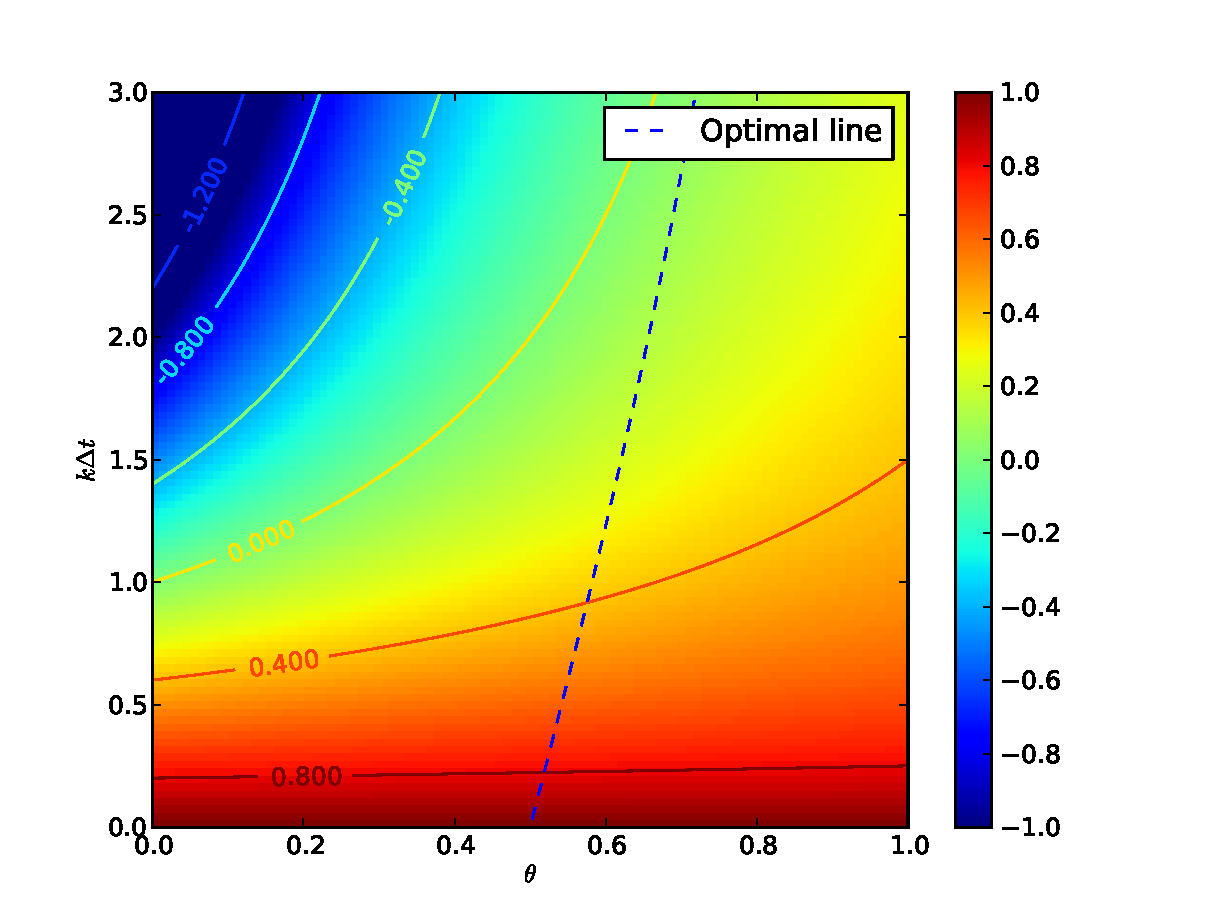
\includegraphics[width=\textwidth]{figures/ampFactor.pdf}
\caption{Figuren viser amplikasjonsfaktor som funksjon av $a\Delta t$ og $\theta$. Linjen som er merket som optimal, er de parameterkombinasjonene som løser $T'=-kT$ eksakt.}
\label{fig:ampFactor}
\end{figure}

\subsection{Artifacts i lys av Amplikasjonsfaktoren}
Det er nyttig å diskutere artifacts i lys av figur \ref{fig:ampFactor}, siden den nesten direkte viser hvordan løsningsrommet ser ut som funksjon av parametrene i de diskrete likningene. Vi ønsker å komme nærme den eksakte løsningen. 

Det vi kan se av åpenbare artifacts, ligger oppe i venstre hjørne av figuren. Der ser vi at vi kan få negative amplikasjonsfaktorer, som tilsvarer oscillerende løsningen, som er en fullstendig ufysisk oppførsel for denne likningen. I verste fall ser vi også oscillerende løsninger som blåser seg opp, de tilsvarer $A<-1$. 

Det som er overraskende, er å se at for store tidssteg kan også Crank-Nicolson-metoden oscillere. 
Backward Euler er kjent for å dempe oscillasjoner, og man ser ut ifra amplikasjonsfaktoren at den gjør det også her. 


\section{Analytisk løsning av $T_t = kT_{xx}$}
Endimensjonal diffusjonslikning har et komplett sett med separable løsninger. Løsningene er på formen:

\begin{equation}
	T(x,t) = T^t(t)T^x(x) = e^{-a^2kt} \begin{cases} \sin{a x} \\ \cos{a x}\end{cases}
\end{equation}

Eventuelt kan man skrive det harmoniske leddet mer generelt:
\begin{equation}
	T(x, t) = e^{-a^2 kt} e^{iax}
\end{equation}

Der $a$ er en vilkårlig konstant, som kan brukes for å lage et komplett sett med løsningsfuksjoner slik at man utspenner hele løsningsrommet. Randbetingelser vil legge restriksjoner på $a$. 

Vi kan utvikle initialbetingelser som en fourierrekke i løsninger av PDEen, og så kjøre ligningen i tid. 

\section{Diskretisering av $T_t = kT_{xx}$}
Vi gjør en sentrert differanse på den romderiverte, og ser på forskjeller mellom FE, BE og CN i den tidsderiverte. 

\begin{equation}
	u^{n+1}
\end{equation}

\section{Feilanalyse og oscillasjonsanalyse for Forward Euler}
Vi begynner med å anta, motivert av den analytiske løsningen, at den numeriske løsningen kan skrives som:
\begin{equation}
	u^n_q = A^ne^{iaq\Delta x}
\end{equation}
Der $n$ angir tidssteg og $q$ angir romsteg. Byttet fra i for å gjøre plass til den imaginære enheten. 

Da kan Forward-Euler-diskretiseringen skrives som:
\begin{equation}
	A^{n+1}e^{iaq\Delta x} = A^ne^{iaq\Delta x} + CA^n(e^{ia(q+1)\Delta x}-2e^{iaq\Delta x} + e^{ia(q-1)\Delta x})
\end{equation}
\begin{equation}
	A^{n+1} = A^n +CA^n(e^{ia\Delta x} + e^{-ia\Delta x} - 2)
\end{equation}
Dette gir at:
\begin{equation}
	A = 1 - 4C\sin^2{\frac{a\Delta x}{2}}
\end{equation}
Eller helt utskrevet:
\begin{equation}
	A = 1 - 4\frac{k\Delta t}{\Delta x^2}\sin^2{\frac{a\Delta x}{2}}
\end{equation}

Siden $\sin^2(x) \leq 1 \ \forall \ x$, så er $A \leq 1$. Vi risikerer imidlertid negative $A$. 

Vi ser først at verste tilfelle for sinus-leddet er $\sin^2{\frac{k\Delta x}{2}} = 1$. Dersom vi setter inn dette, blir stabilitetskriteriet for å ha $|A| < 1$:

\begin{equation}
	1 - 4\frac{k\Delta t}{\Delta x^2} > -1
\end{equation}
\begin{equation}
	\frac{k\Delta t}{\Delta x^2} < \frac{1}{2}
\end{equation}

Artifacts med denne metoden vil være at løsningen oscillerer.

Man kan sette opp et alternativt krav, nemlig det for å unngå oscillasjoner: 
\begin{equation}
	1 - 4\frac{k \Delta t}{\Delta x^2} > 0 
\end{equation}
\begin{equation}
	\frac{k\Delta t}{\Delta x^2} < \frac{1}{4}
\end{equation}
Tallet $a$ i sinusleddet er noe vi ikke har kontroll på. Det vil si at vi vet at vi kan få oscillatorisk oppførsel for enkelte a. 

En løsning av et problem vil stort sett være en lineærkombinasjon av løsningsfunksjoner, med forskjellige $a$. I denne oppgaven ser vi på ekstremtilfellet med en diskontinuitet, som i prinsippet krever en uendelig rekke for å representeres. Vi får også et gibbs-problem. 

Store $a$ svarer til høyfrekvente løsninger, mens små $a$ svarer til lavfrekvente. De lavfrekvente vil typisk bygge opp en hovedform, mens de høyfrekvente kan skape oscillasjoner om hovedtrenden. Dette skjer i diffusjonslikningen når man begynner med en diskontinuitet, og får $A<0$ for store $a$. Løsningen av den diskrete likningen vil da oscillere for korte bølger.

\section{Feilanalyse for CN og BE}
Her gjør vi ikke hele jobben med å utlede satbilitetskravet, men ser heller direkte på amplifikasjonsfaktoren for de numeriske skjemaene. 

\begin{center}
Backward Euler
\begin{equation}
	A = (1  + 4C\sin^2{\frac{k\Delta x}{2}})^{-1}
\end{equation}
Crank-Nicolson
\begin{equation}
	A = \frac{ 1 - 2C\sin^2p}{1 + 2C\sin^2p}
\end{equation}
\end{center}

Vi ser at $A \in (0, 1]$ for Backward Euler, så her forventer vi ingen artifacts. For Crank-Nicolson 

***Si litt mer om diffusjonslikningen***
***Sammenlikne feilanalysen***

\end{document}

